% CaelumFusion VGA Rendering Configuration and Control Map
% Source-aligned engineering design reference for the Basys-3 VGA path.
%
% This document is intentionally VGA-only.  It does not describe HDMI, TMDS,
% DisplayPort, or any digital video encoder path.

\documentclass[12pt,letterpaper,final,onecolumn,titlepage]{article}

%------------------------------------------------------------------------------
% Mathematics and symbols
%------------------------------------------------------------------------------
\usepackage{amsmath}
\usepackage{amssymb}

%------------------------------------------------------------------------------
% Page geometry, typography, and structure
%------------------------------------------------------------------------------
\usepackage[margin=0.82in]{geometry}
\usepackage[T1]{fontenc}
\usepackage[utf8]{inputenc}
\usepackage{microtype}
\usepackage{enumitem}
\usepackage{fancyhdr}
\usepackage{lastpage}

%------------------------------------------------------------------------------
% Figures, tables, colors, and diagrams
%------------------------------------------------------------------------------
\usepackage{graphicx}
\usepackage{float}
\usepackage{booktabs}
\usepackage{array}
\usepackage{tabularx}
\usepackage{longtable}
\usepackage[dvipsnames]{xcolor}
\usepackage{tikz}
\usetikzlibrary{arrows.meta,calc,fit,positioning,shapes.geometric}

%------------------------------------------------------------------------------
% Hyperlinks
%------------------------------------------------------------------------------
\usepackage[hidelinks]{hyperref}

%------------------------------------------------------------------------------
% Engineering notation
%------------------------------------------------------------------------------
\DeclareRobustCommand{\rtl}[1]{\texttt{\detokenize{#1}}}
\DeclareRobustCommand{\sig}[1]{\texttt{\detokenize{#1}}}
\DeclareRobustCommand{\param}[1]{\texttt{\detokenize{#1}}}
\DeclareRobustCommand{\file}[1]{\texttt{\detokenize{#1}}}
\DeclareRobustCommand{\view}[1]{\textsc{\detokenize{#1}}}
\DeclareRobustCommand{\bits}[1]{\texttt{\detokenize{#1}}}

\newcolumntype{Y}{>{\raggedright\arraybackslash}X}
\newcolumntype{L}[1]{>{\raggedright\arraybackslash}p{#1}}
\newcolumntype{C}[1]{>{\centering\arraybackslash}p{#1}}

\setlength{\parindent}{0pt}
\setlength{\parskip}{5pt}
\renewcommand{\arraystretch}{1.16}
\setlist[itemize]{leftmargin=1.45em,itemsep=2pt,topsep=3pt}
\setlist[enumerate]{leftmargin=1.65em,itemsep=2pt,topsep=3pt}

%------------------------------------------------------------------------------
% Color palette
%------------------------------------------------------------------------------
\definecolor{CFInk}{HTML}{0B1320}
\definecolor{CFPanel}{HTML}{172A3A}
\definecolor{CFBlue}{HTML}{2868A6}
\definecolor{CFCyan}{HTML}{00A8C8}
\definecolor{CFGreen}{HTML}{238B45}
\definecolor{CFAmber}{HTML}{C47F00}
\definecolor{CFOrange}{HTML}{D95F02}
\definecolor{CFRed}{HTML}{C92A2A}
\definecolor{CFPurple}{HTML}{6A51A3}
\definecolor{CFGray}{HTML}{667085}
\definecolor{CFGrid}{HTML}{D7DEE8}
\definecolor{CFLight}{HTML}{F4F7FB}

%------------------------------------------------------------------------------
% TikZ styles
%------------------------------------------------------------------------------
\tikzset{
  cfBlock/.style={
    rectangle, rounded corners=2pt, draw=#1!80!black, fill=#1!12,
    align=center, text=black, minimum width=2.75cm, minimum height=0.78cm,
    inner sep=4pt, font=\small
  },
  cfBlock/.default=CFBlue,
  cfSmall/.style={
    rectangle, rounded corners=2pt, draw=#1!80!black, fill=#1!10,
    align=center, text=black, minimum width=2.1cm, minimum height=0.58cm,
    inner sep=3pt, font=\scriptsize
  },
  cfSmall/.default=CFBlue,
  cfState/.style={
    rectangle, rounded corners=2pt, draw=#1!85!black, fill=#1!13,
    align=center, text=black, minimum width=2.45cm, minimum height=0.78cm,
    inner sep=4pt, font=\scriptsize
  },
  cfState/.default=CFGreen,
  cfMux/.style={
    diamond, aspect=2.1, draw=CFOrange!90!black, fill=CFOrange!13,
    align=center, inner sep=1.2pt, font=\scriptsize
  },
  cfFrame/.style={
    rounded corners=5pt, draw=#1!80!black, fill=none,
    line width=0.45pt, inner sep=6pt
  },
  cfFrame/.default=CFGrid,
  cfArrow/.style={-{Latex[length=2.1mm]}, draw=CFBlue!90!black, line width=0.62pt},
  cfCtrl/.style={-{Latex[length=2.1mm]}, draw=CFAmber!90!black, line width=0.62pt},
  cfOverride/.style={-{Latex[length=2.1mm]}, draw=CFRed!85!black, line width=0.78pt},
  cfDashed/.style={-{Latex[length=2.0mm]}, draw=CFGray!90!black, line width=0.55pt, dashed},
  cfLayer/.style={
    rectangle, rounded corners=2pt, draw=#1!85!black, fill=#1!15,
    minimum width=8.9cm, minimum height=0.55cm, align=center, font=\small
  },
  cfLayer/.default=CFBlue
}

%------------------------------------------------------------------------------
% Screen-layout helper macros
%------------------------------------------------------------------------------
\newcommand{\screenframe}[1]{%
  \fill[CFInk] (0,0) rectangle (640,480);
  \draw[white, line width=0.75pt] (0,0) rectangle (640,480);
  \draw[CFGrid!40, line width=0.16pt, step=80] (0,0) grid (640,480);
  \node[anchor=north west, text=white, font=\scriptsize] at (8,8) {#1};
  \node[anchor=north east, text=CFGrid, font=\tiny] at (634,8) {640x480 active};
}

\newcommand{\screenrect}[6]{%
  \draw[draw=#5!88!black, fill=#5!58, line width=0.45pt]
    (#1,#2) rectangle ++(#3,#4);
  \node[align=center, text=white, font=\tiny] at ({#1 + #3/2},{#2 + #4/2}) {#6};
}

\newcommand{\screendashedrect}[6]{%
  \draw[draw=#5!88!black, fill=#5!28, line width=0.45pt, dashed]
    (#1,#2) rectangle ++(#3,#4);
  \node[align=center, text=white, font=\tiny] at ({#1 + #3/2},{#2 + #4/2}) {#6};
}

%------------------------------------------------------------------------------
% Header/footer
%------------------------------------------------------------------------------
\pagestyle{fancy}
\fancyhf{}
\setlength{\headheight}{15pt}
\lhead{CaelumFusion}
\rhead{VGA Rendering Configuration}
\cfoot{\thepage\ of \pageref{LastPage}}

\title{
  \vspace{0.45in}
  \textbf{CaelumFusion VGA Rendering Configuration and Control Map}\\[0.65em]
  \large Engineering Design Reference
}
\author{CaelumFusion Flight Control System}
\date{Draft updated July 6, 2026}

\begin{document}
\maketitle

\begin{center}
\fbox{\begin{minipage}{0.92\linewidth}
\textbf{Source and scope statement.} This document describes the active
CaelumFusion Basys-3 VGA rendering path.  The board-facing display contract is
\sig{vga_hsync}, \sig{vga_vsync}, and \sig{vga_rgb[11:0]} only.  HDMI, TMDS,
DisplayPort, DVI, and digital-video encoder behavior are outside the scope of
this control map.
\end{minipage}}
\end{center}

\tableofcontents
\listoffigures
\listoftables
\newpage

\section{Scope and Purpose}

This document specifies how the CaelumFusion VGA renderer is configured,
selected, composed, and driven to the Basys-3 analog VGA connector.  It is
written as an engineering control artifact: each display mode is tied to an RTL
view state, each operator control is tied to a board signal, and each visible
fallback behavior is tied to an implemented default or a compile-time option.

The document covers:
\begin{itemize}
  \item available display views and rendering modes;
  \item buttons, switches, and control-register style inputs that influence view
        selection;
  \item view-selection priority rules and default/fallback display behavior;
  \item widget enable controls, layer priorities, and compositor behavior;
  \item viewport locations, color conventions, and telemetry fields shown in
        each mode;
  \item debugging usefulness and known rendering limitations.
\end{itemize}

\section{Authoritative Source Inputs}

The contracts below are grounded in the active project files listed in
Table~\ref{tab:sources}.  Older report artifacts and unrelated HDMI documents
are useful style references only; they are not treated as implementation
evidence for CaelumFusion.

\begin{table}[H]
\caption{Source files used as the implementation contract.}
\label{tab:sources}
\footnotesize
\begin{tabularx}{\linewidth}{L{0.41\linewidth} Y}
\toprule
\textbf{Source} & \textbf{Relevant contract} \\
\midrule
\file{caelumfusion_top_vga.v} &
Board-facing integration top.  Owns raw controls, synchronization, debounce,
sensor publication, render-control wrapper instantiation, pixel-clock path, and
final VGA pins. \\
\file{caelumfusion_vga_render_control.v} &
Legal view states, next/previous/direct selection, invalid-direct-view latch,
legacy hold priority, self-test enable, compass-page enable, and HUD page
select. \\
\file{flight_viz_suite_top.v} &
Live-vs-self-test visualization source selection, SYS-to-PIX semantic transfer,
history control, and flight visualizer instantiation. \\
\file{flight_visualizer_pix.v} &
640x480 PIX-domain renderer, frame-boundary visual commit, fixed layout,
sensor diagnostic page, telemetry text inputs, history plots, and RGB output. \\
\file{flight_vga_page_mux_pix.v} &
Final primary-HUD versus sensor-diagnostic page selection, text overlay
priority, and active-video blacking. \\
\file{planar_compass_truth_page_vga.v} &
Optional full-screen compass/MAG truth page overlay that replaces VGA RGB while
passing timing through. \\
\file{Basys-3-Master.xdc} &
Board pin map, switch/button map, VGA RGB bit ordering, and scoped false-path
constraints for asynchronous board inputs. \\
\bottomrule
\end{tabularx}
\end{table}

\section{Notation and Configuration Model}

Let \(V_s\) be the registered SYS-domain view state in
\sig{view_sel_sys}.  Let \(V_e\) be the effective view after legacy holds have
been applied in \sig{view_effective_sys}.  Let \(P\) be the HUD-renderer page
select driven into \sig{flight_visualizer_pix}.  Let \(R(x,y)\) be the final
12-bit RGB value driven for active pixel coordinate \((x,y)\).  Let \(D\) be
the direct-view request ID sampled by the board-level direct-select latch.

The renderer separates three kinds of control:
\begin{itemize}
  \item \textbf{Compile-time inclusion}: page-inclusion parameters decide
        whether optional compass-truth and sensor-diagnostic renderer logic
        exists in the bitstream.
  \item \textbf{Runtime view selection}: buttons, direct-select inputs, and
        legacy holds decide which included renderer path is selected.
  \item \textbf{Switch-encoded navigation}: in the active Basys-3 top, the
        encoded selector is enabled.  Therefore \(D\) is derived from the
        synchronized SW13:SW11 switch triplet and BTNR is the load strobe for
        deterministic random access into the renderer set, but only when SW3
        MAG1 bench mode and SW2+SW6 diagnostic fault injection are inactive.
  \item \textbf{Telemetry validity}: visible colors and widgets reflect
        validity, age, status, freshness, and sequence fields without changing
        the selected view.
\end{itemize}

\section{Board-Level VGA Contract}

\subsection{Physical Interface}

The Basys-3 output is analog VGA driven from 12 RGB pins and two sync pins.
Table~\ref{tab:vga-pins} summarizes the display port contract.

\begin{table}[H]
\caption{Board-facing VGA output contract.}
\label{tab:vga-pins}
\small
\begin{tabularx}{\linewidth}{L{0.22\linewidth} L{0.20\linewidth} Y}
\toprule
\textbf{RTL signal} & \textbf{Board mapping} & \textbf{Meaning} \\
\midrule
\sig{vga_hsync} & package pin \sig{P19} & Horizontal synchronization, polarity from the VGA timing generator. \\
\sig{vga_vsync} & package pin \sig{R19} & Vertical synchronization, polarity from the VGA timing generator. \\
\sig{vga_rgb[11:8]} & Basys-3 red resistor ladder & 4-bit red channel. \\
\sig{vga_rgb[7:4]} & Basys-3 green resistor ladder & 4-bit green channel. \\
\sig{vga_rgb[3:0]} & Basys-3 blue resistor ladder & 4-bit blue channel. \\
\bottomrule
\end{tabularx}
\end{table}

The active coordinate convention is upper-left origin, \(x=0\ldots639\) and
\(y=0\ldots479\).  The display path is designed around 640 by 480 active video
with a 25 MHz pixel clock generated from the board clock.

\subsection{Button Map}

\begin{table}[H]
\caption{Button inputs that affect VGA rendering.}
\label{tab:buttons}
\small
\begin{tabularx}{\linewidth}{L{0.14\linewidth} L{0.28\linewidth} Y}
\toprule
\textbf{Board control} & \textbf{RTL signal} & \textbf{Rendering behavior} \\
\midrule
BTNC & \sig{rst} & Global reset.  Resets registered view state to the safe configured reset view. \\
BTNU & \sig{btn_page_raw} & Debounced next-view pulse.  Cycles the registered view forward. \\
BTND & \sig{btn_prev_raw} & Debounced previous-view pulse.  Cycles the registered view backward. \\
BTNR & \sig{btn_direct_compass_raw} & Debounced direct-select latch.  In the active encoded-selector build it loads the synchronized SW13:SW11 view ID only while SW3 MAG1 bench mode and SW2+SW6 diagnostic fault injection are inactive.  If \param{USE_SWITCH_ENCODED_VIEW_SELECT} is set to zero in a future build, BTNR reverts to the fixed compass/MAG truth request. \\
BTNL & unused & Intentionally not part of the current top-level render-control contract. \\
\bottomrule
\end{tabularx}
\end{table}

\subsection{Switch Map}

Board switches affect both view selection and visible telemetry content.  A
switch can only enable logic that is present in the bitstream.

\begin{longtable}{L{0.13\linewidth} L{0.30\linewidth} L{0.47\linewidth}}
\caption{Switch inputs relevant to VGA rendering and diagnostic content.}
\label{tab:switches}\\
\toprule
\textbf{Switch} & \textbf{RTL signal} & \textbf{Rendering effect} \\
\midrule
\endfirsthead
\toprule
\textbf{Switch} & \textbf{RTL signal} & \textbf{Rendering effect} \\
\midrule
\endhead
SW0 & \sig{sw_arm_raw} & Authority/status visualization arm input. \\
SW1 & \sig{sw_policy_enable_raw} & Policy-enable evidence for authority/status visualization. \\
SW2 & \sig{sw_selftest_raw} & Holds self-test HUD stimulus high unless masked by the SW2+SW6 diagnostic fault-injection combination. \\
SW3 & \sig{sw_mag1_bench_raw} & Enables synthetic MAG1 bench source when compiled. \\
SW4 & \sig{sw_compass_page_raw} & Legacy hold for compass/MAG evidence page. \\
SW5 & \sig{sw_history_freeze_raw} & Freezes HUD history-ring writes for inspection while keeping display timing active. \\
SW6 & \sig{sw_log_diag_raw} & Enables black-box/log diagnostic behavior when compiled; with SW2 also selects diagnostic fault injection. \\
SW7 & \sig{sw_lis3dh_i2c_acc_raw} & Runtime gate for LIS3DH I2C accelerometer publication when compiled. \\
SW8 & \sig{sw_adxl362_spi_acc_raw} & Runtime gate for ADXL362/Pmod ACL2 SPI accelerometer publication when compiled. \\
SW9 & \sig{sw_cmps2_mmc3416_mag_raw} & Runtime gate for CMPS2/MMC34160PJ magnetometer publication when compiled. \\
SW10 & \sig{sw_pmon1_pwr_raw} & Runtime gate for PMON1 power telemetry publication when compiled. \\
SW11--SW13 & \sig{sw_mag1_offset_*_raw} & Apply synthetic MAG1 offset components when the MAG1 bench source is enabled.  With SW2+SW6 they select diagnostic fault class.  In the active encoded-selector build, these same synchronized levels form \sig{view_direct_id_sys[2:0]} as \sig{\{SW13,SW12,SW11\}} only while SW3 MAG1 bench mode and SW2+SW6 fault injection are inactive. \\
SW14 & \sig{sw_compass_default_raw} & Companion legacy hold for compass/MAG evidence page. \\
SW15 & \sig{sw_ext_i2c_raw} & Optional shared-I2C extension group enable for extension telemetry. \\
\bottomrule
\end{longtable}

\section{Rendering-to-VGA Pipeline}

\subsection{Pipeline Overview}

Figure~\ref{fig:pipeline} shows the implemented rendering path from raw board
controls and SYS-domain telemetry to final VGA output.  The drawing separates
selection control, semantic telemetry publication, renderer selection, and final
RGB composition.

\begin{figure}[H]
\centering
\resizebox{\linewidth}{!}{%
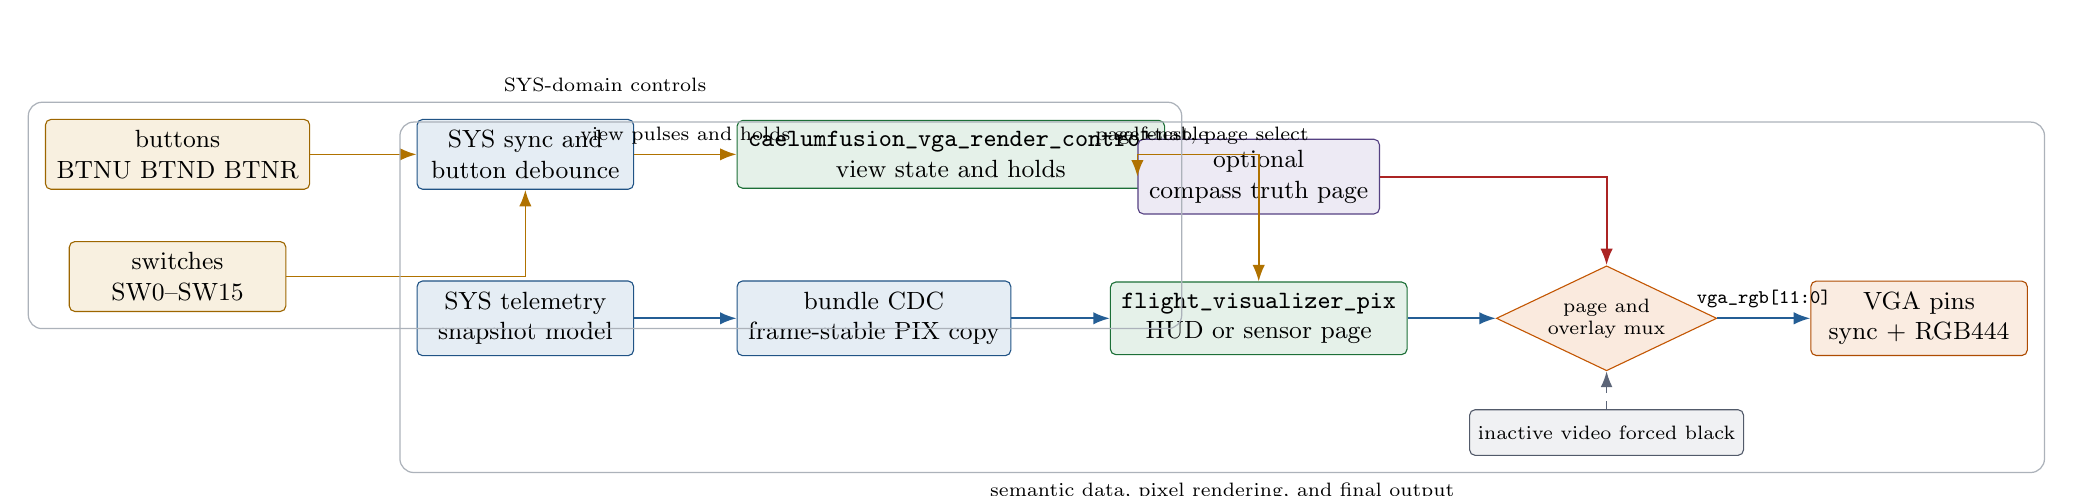
\begin{tikzpicture}[node distance=0.85cm and 1.05cm]
  \node[cfBlock=CFAmber] (buttons) {buttons\\BTNU BTND BTNR};
  \node[cfBlock=CFAmber, below=0.65cm of buttons] (switches) {switches\\SW0--SW15};
  \node[cfBlock=CFBlue, right=1.35cm of buttons] (sync) {SYS sync and\\button debounce};
  \node[cfBlock=CFGreen, right=1.30cm of sync] (control) {\file{caelumfusion_vga_render_control}\\view state and holds};

  \node[cfBlock=CFBlue, below=1.15cm of sync] (telemetry) {SYS telemetry\\snapshot model};
  \node[cfBlock=CFBlue, right=1.30cm of telemetry] (cdc) {bundle CDC\\frame-stable PIX copy};

  \node[cfBlock=CFGreen, right=1.25cm of cdc] (hud) {\file{flight_visualizer_pix}\\HUD or sensor page};
  \node[cfBlock=CFPurple, above=0.85cm of hud] (truth) {optional\\compass truth page};
  \node[cfMux, right=1.12cm of hud] (mux) {page and\\overlay mux};
  \node[cfBlock=CFOrange, right=1.18cm of mux] (vga) {VGA pins\\sync + RGB444};

  \draw[cfCtrl] (buttons.east) -- (sync.west);
  \draw[cfCtrl] (switches.east) -| (sync.south);
  \draw[cfCtrl] (sync.east) -- node[above, font=\scriptsize]{view pulses and holds} (control.west);
  \draw[cfCtrl] (control.east) -| node[pos=0.25, above, font=\scriptsize]{self-test, page select} (hud.north);
  \draw[cfCtrl] (control.east) -| node[pos=0.24, above, font=\scriptsize]{page enable} (truth.west);

  \draw[cfArrow] (telemetry.east) -- (cdc.west);
  \draw[cfArrow] (cdc.east) -- (hud.west);
  \draw[cfArrow] (hud.east) -- (mux.west);
  \draw[cfOverride] (truth.east) -| (mux.north);
  \draw[cfArrow] (mux.east) -- node[above, font=\scriptsize]{\sig{vga_rgb[11:0]}} (vga.west);

  \node[cfSmall=CFGray, below=0.48cm of mux] (black) {inactive video forced black};
  \draw[cfDashed] (black.north) -- (mux.south);

  \node[cfFrame=CFGrid, fit=(buttons)(switches)(sync)(control), label={[font=\scriptsize]above:SYS-domain controls}] {};
  \node[cfFrame=CFGrid, fit=(telemetry)(cdc)(hud)(truth)(mux)(vga)(black), label={[font=\scriptsize]below:semantic data, pixel rendering, and final output}] {};
\end{tikzpicture}}
\caption[CaelumFusion VGA rendering pipeline]{CaelumFusion VGA rendering pipeline.  Control inputs are synchronized in SYS, view-selection state drives renderer enables, telemetry is transferred into PIX through a frame-stable bundle, and final RGB is selected by the page/compositor path.}
\label{fig:pipeline}
\end{figure}

\subsection{Final Output Function}

The primary PIX renderer produces \sig{hud_rgb}, optional
\sig{sensor_diag_rgb}, and text overlay RGB.  The page mux implements the
following priority inside active video:
\[
R_{\mathrm{hud}}(x,y)=
\begin{cases}
0, & \text{if inactive video},\\
R_{\mathrm{text}}(x,y), & \text{if text overlay is active and sensor page is not selected},\\
R_{\mathrm{sensor}}(x,y), & \text{if sensor diagnostic page is selected},\\
R_{\mathrm{base}}(x,y), & \text{otherwise}.
\end{cases}
\]
When the optional compass truth page is enabled and selected, it replaces the
HUD RGB stream at the wrapper level while preserving the VGA timing path.

\section{VGA View-Selection Logic}

\subsection{Legal View States}

\begin{table}[H]
\caption{Legal render-view states.}
\label{tab:views}
\small
\begin{tabularx}{\linewidth}{L{0.23\linewidth} C{0.09\linewidth} L{0.20\linewidth} Y}
\toprule
\textbf{View state} & \textbf{ID} & \textbf{Compile-time gate} & \textbf{Visible behavior} \\
\midrule
\sig{VIEW_FLIGHT_HUD} & \bits{3'd0} & always legal & Normal flight HUD using live telemetry bundle. \\
\sig{VIEW_COMPASS_TRUTH} & \bits{3'd1} & compass page included & Full-screen compass/MAG truth diagnostic page.  Illegal direct requests are rejected when \param{ENABLE_COMPASS_TRUTH_PAGE} is zero. \\
\sig{VIEW_SELFTEST_HUD} & \bits{3'd2} & always legal & Normal HUD renderer driven by self-test stimulus. \\
\sig{VIEW_SENSOR_DIAG} & \bits{3'd3} & visible page optional & HUD-renderer diagnostic page for sensor, extension, navigation, and wind evidence; falls back to primary HUD RGB when \param{ENABLE_SENSOR_DIAG_PAGE} is zero. \\
\sig{VIEW_SCIENCE_EXPLAIN} & \bits{3'd4} & science pages included & Compact physics/environment evidence overlay. \\
\sig{VIEW_SCIENCE_WIND} & \bits{3'd5} & science pages included & Compact wind triangle and dispersion evidence overlay. \\
\sig{VIEW_SCIENCE_INTEGRITY} & \bits{3'd6} & science pages included & Compact sensor-integrity correlation overlay. \\
\bits{3'd7} & reserved & illegal & Direct requests are rejected and latch \sig{cfg_invalid_view_sys}. \\
\bottomrule
\end{tabularx}
\end{table}

\subsection{Navigation State Machine}

Figure~\ref{fig:navigation} shows the legacy view navigation contract.  In the
current RTL, next cycles \view{flight-hud} to \view{sensor-diag}, then through
the science pages when \param{ENABLE_SCIENCE_PAGES} is nonzero, then through
\view{compass-truth} when \param{ENABLE_COMPASS_TRUTH_PAGE} is nonzero, then to
\view{selftest-hud} and back to \view{flight-hud}.  Disabled page families are
skipped.

\begin{figure}[H]
\centering
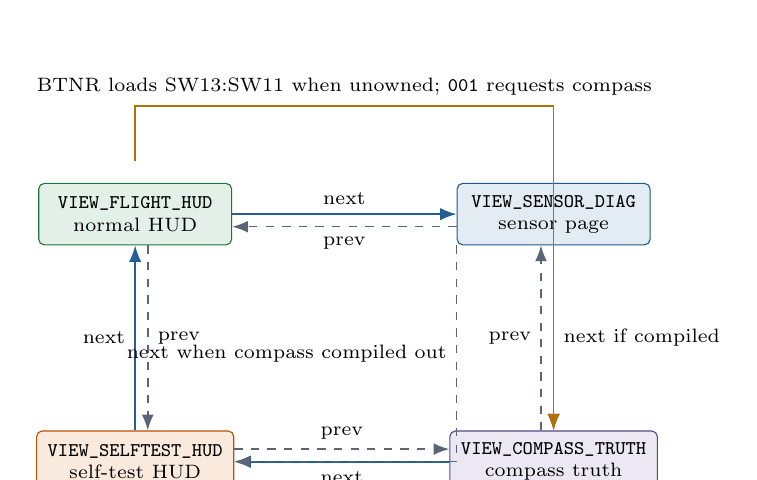
\begin{tikzpicture}[node distance=2.35cm and 2.85cm]
  \node[cfState=CFGreen] (hud) {\sig{VIEW_FLIGHT_HUD}\\normal HUD};
  \node[cfState=CFBlue, right=of hud] (diag) {\sig{VIEW_SENSOR_DIAG}\\sensor page};
  \node[cfState=CFPurple, below=of diag] (truth) {\sig{VIEW_COMPASS_TRUTH}\\compass truth};
  \node[cfState=CFOrange, below=of hud] (self) {\sig{VIEW_SELFTEST_HUD}\\self-test HUD};

  \draw[cfArrow] (hud.east) -- node[above, font=\scriptsize]{next} (diag.west);
  \draw[cfArrow] (diag.south) -- node[right, font=\scriptsize]{next if compiled} (truth.north);
  \draw[cfArrow] (truth.west) -- node[below, font=\scriptsize]{next} (self.east);
  \draw[cfArrow] (self.north) -- node[left, font=\scriptsize]{next} (hud.south);

  \draw[cfDashed] ([yshift=-0.16cm]diag.west) -- node[below, font=\scriptsize]{prev} ([yshift=-0.16cm]hud.east);
  \draw[cfDashed] ([xshift=-0.16cm]truth.north) -- node[left, font=\scriptsize]{prev} ([xshift=-0.16cm]diag.south);
  \draw[cfDashed] ([yshift=0.16cm]self.east) -- node[above, font=\scriptsize]{prev} ([yshift=0.16cm]truth.west);
  \draw[cfDashed] ([xshift=0.16cm]hud.south) -- node[right, font=\scriptsize]{prev} ([xshift=0.16cm]self.north);

  \draw[cfDashed] (diag.south west) |- node[pos=0.25, left, font=\scriptsize]{next when compass compiled out} (self.east);
  \draw[cfCtrl] ([yshift=0.28cm]hud.north) -- ++(0,0.70) -| node[pos=0.25, above, font=\scriptsize]{BTNR loads SW13:SW11 when unowned; \bits{001} requests compass} (truth.north);
\end{tikzpicture}
\caption[VGA view-selection navigation]{VGA view-selection navigation.  Solid arrows are normal next transitions with the optional compass page present; dashed arrows show reverse and disabled-feature behavior.}
\label{fig:navigation}
\end{figure}

\subsection{Switch-Encoded Direct Selection}

The active board top enables switch-encoded view selection.  With that
parameter nonzero, the top-level direct request is:
\[
\begin{aligned}
\mathrm{view\_direct\_valid\_sys} &= \text{rising edge of BTNR},\\
\mathrm{view\_direct\_id\_sys[2:0]} &=
\begin{cases}
\{\text{SW13},\text{SW12},\text{SW11}\}, & \text{SW3=0 and not(SW2+SW6)}\\
\bits{3'b111}, & \text{SW3=1 or SW2+SW6 fault injection active.}
\end{cases}
\end{aligned}
\]
The switches are synchronized continuously in SYS; they do not update
\sig{view_sel_sys} by themselves.  BTNR is the latch edge that converts the
visible physical switch pattern into a one-cycle direct-view request.  For
example, SW13, SW12, and SW11 high presents \bits{3'b111}; pressing BTNR while
SW3 is low and SW2+SW6 fault injection is inactive requests that hard-defined
direct ID.  Because \bits{3'b111} is reserved, the wrapper rejects it, holds the
current registered view, and sets \sig{cfg_invalid_view_sys}.  The same
reserved request is generated automatically whenever MAG1 bench mode or
diagnostic fault injection owns SW11--SW13, giving the bench a deterministic
negative test for invalid view encodings and preventing accidental navigation.

\begin{table}[H]
\caption{Optional SW13:SW11 direct-view encodings.}
\label{tab:switch-encoded-view}
\small
\begin{tabularx}{\linewidth}{C{0.18\linewidth} L{0.28\linewidth} Y}
\toprule
\textbf{SW13:SW11} & \textbf{Requested view ID} & \textbf{Effect when BTNR is pressed} \\
\midrule
\bits{3'b000} & \sig{VIEW_FLIGHT_HUD} & Selects the normal live-telemetry HUD. \\
\bits{3'b001} & \sig{VIEW_COMPASS_TRUTH} & Selects the compass/MAG truth page when compiled in; otherwise rejected as an unavailable direct request. \\
\bits{3'b010} & \sig{VIEW_SELFTEST_HUD} & Selects the normal HUD renderer with self-test stimulus. \\
\bits{3'b011} & \sig{VIEW_SENSOR_DIAG} & Selects the sensor diagnostic view; if its page logic is compiled out, the registered view changes but visible RGB falls back to the primary HUD. \\
\bits{3'b100} & \sig{VIEW_SCIENCE_EXPLAIN} & Selects the compact physics/environment evidence page when science pages are compiled in; otherwise rejected. \\
\bits{3'b101} & \sig{VIEW_SCIENCE_WIND} & Selects the compact wind triangle / dispersion evidence page when science pages are compiled in; otherwise rejected. \\
\bits{3'b110} & \sig{VIEW_SCIENCE_INTEGRITY} & Selects the compact sensor-integrity correlation page when science pages are compiled in; otherwise rejected. \\
\bits{3'b111} & reserved & Rejected by \file{caelumfusion_vga_render_control.v}; \sig{view_sel_sys} is held and \sig{cfg_invalid_view_sys} latches. \\
\bottomrule
\end{tabularx}
\end{table}

The selector intentionally reuses SW11--SW13 as a bench navigation aid.  Those
same switches also carry MAG1 bench-offset and fault-class meaning, so the RTL
assigns ownership to MAG1 bench mode and diagnostic fault injection.  For clean
direct navigation, clear SW3 and clear either SW2 or SW6, set SW13:SW11 to the
desired direct ID, press BTNR, then restore the MAG1 bench or diagnostic
fault-injection switches for the intended scenario.

\subsection{Priority Rules}

The effective view is selected by the deterministic priority chain in
Table~\ref{tab:priority}.  The first true condition wins.

\begin{table}[H]
\caption{Effective-view priority.}
\label{tab:priority}
\small
\begin{tabularx}{\linewidth}{C{0.12\linewidth} L{0.38\linewidth} Y}
\toprule
\textbf{Priority} & \textbf{Condition} & \textbf{Effective view} \\
\midrule
1 & Compass legacy hold is high and compass page logic is present & \sig{VIEW_COMPASS_TRUTH} \\
2 & Self-test legacy hold is high & \sig{VIEW_SELFTEST_HUD} \\
3 & No hold has priority & registered \sig{view_sel_sys} \\
\bottomrule
\end{tabularx}
\end{table}

The registered view state \(V_s\) changes only on legal direct requests or
debounced next/previous pulses.  Illegal direct requests do not change
\sig{view_sel_sys}; they set \sig{cfg_invalid_view_sys}.  The current board top
ties \sig{cfg_invalid_view_clear_sys} low, so reset is the only board-level
clear path for that latch unless a future visible clear control is added.
Legacy holds are applied after the registered direct-selection state, so SW4 or
SW14 can still force the effective compass page and SW2 can still force
self-test even when the encoded selector has loaded another legal view.

\section{Control-to-Renderer Mapping}

Figure~\ref{fig:control-map} maps physical controls and configuration fields to
the renderer outputs they affect.  The diagram uses orthogonal routes to show
the split between registered view navigation, legacy holds, widget gates, and
final VGA selection.

\begin{figure}[H]
\centering
\resizebox{\linewidth}{!}{%
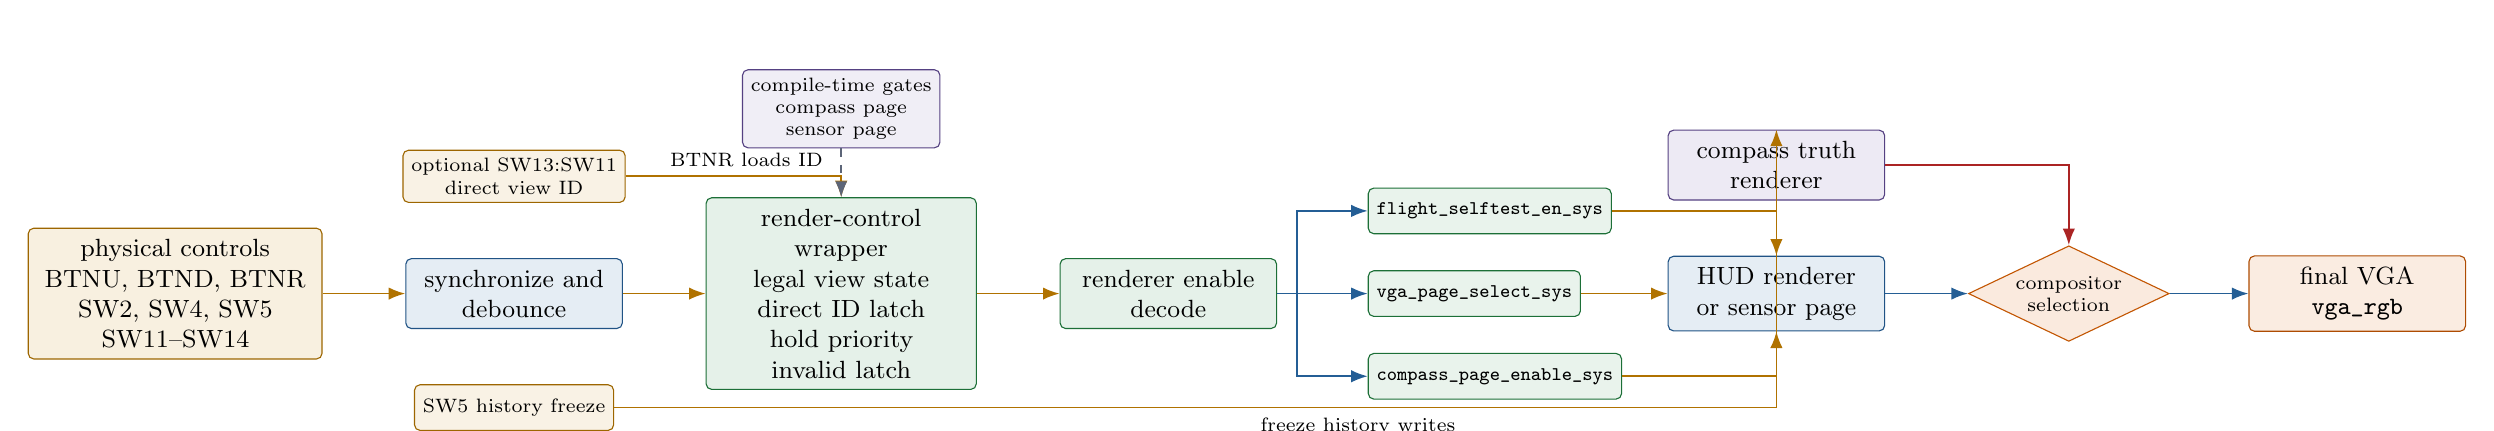
\begin{tikzpicture}[node distance=0.85cm and 1.05cm]
  \node[cfBlock=CFAmber, text width=3.45cm] (phys) {physical controls\\BTNU, BTND, BTNR\\SW2, SW4, SW5\\SW11--SW14};
  \node[cfBlock=CFBlue, right=1.05cm of phys] (sync) {synchronize and\\debounce};
  \node[cfBlock=CFGreen, right=1.05cm of sync, text width=3.15cm] (control) {render-control wrapper\\legal view state\\direct ID latch\\hold priority\\invalid latch};
  \node[cfBlock=CFGreen, right=1.05cm of control] (decode) {renderer enable\\decode};

  \node[cfSmall=CFGreen, right=1.15cm of decode, yshift=1.05cm] (selfen) {\sig{flight_selftest_en_sys}};
  \node[cfSmall=CFGreen, right=1.15cm of decode] (page) {\sig{vga_page_select_sys}};
  \node[cfSmall=CFGreen, right=1.15cm of decode, yshift=-1.05cm] (compass) {\sig{compass_page_enable_sys}};

  \node[cfBlock=CFBlue, right=1.10cm of page] (hud) {HUD renderer\\or sensor page};
  \node[cfBlock=CFPurple, above=0.70cm of hud] (truth) {compass truth\\renderer};
  \node[cfMux, right=1.05cm of hud] (mux) {compositor\\selection};
  \node[cfBlock=CFOrange, right=1.00cm of mux] (vga) {final VGA\\\sig{vga_rgb}};

  \node[cfSmall=CFPurple, above=0.62cm of control] (params) {compile-time gates\\compass page\\sensor page};
  \node[cfSmall=CFAmber, below=0.70cm of sync] (freeze) {SW5 history freeze};
  \node[cfSmall=CFAmber, above=0.70cm of sync] (directid) {optional SW13:SW11\\direct view ID};

  \draw[cfCtrl] (phys.east) -- (sync.west);
  \draw[cfCtrl] (sync.east) -- (control.west);
  \draw[cfCtrl] (directid.east) -| node[pos=0.28, above, font=\scriptsize]{BTNR loads ID} (control.north);
  \draw[cfDashed] (params.south) -- (control.north);
  \draw[cfCtrl] (control.east) -- (decode.west);

  \draw[cfArrow] (decode.east) -- ++(0.25,0) |- (selfen.west);
  \draw[cfArrow] (decode.east) -- (page.west);
  \draw[cfArrow] (decode.east) -- ++(0.25,0) |- (compass.west);
  \draw[cfCtrl] (selfen.east) -| (hud.north);
  \draw[cfCtrl] (page.east) -- (hud.west);
  \draw[cfCtrl] (compass.east) -| (truth.north);
  \draw[cfCtrl] (freeze.east) -| node[pos=0.32, below, font=\scriptsize]{freeze history writes} (hud.south);

  \draw[cfArrow] (hud.east) -- (mux.west);
  \draw[cfOverride] (truth.east) -| (mux.north);
  \draw[cfArrow] (mux.east) -- (vga.west);
\end{tikzpicture}}
\caption[Control-to-renderer mapping]{Control-to-renderer mapping from board controls and compile-time gates to self-test selection, sensor diagnostic page selection, compass truth overlay, and final VGA output.}
\label{fig:control-map}
\end{figure}

\section{Rendering Modes and Telemetry Widgets}

\small
\begin{longtable}{L{0.18\linewidth} L{0.23\linewidth} L{0.26\linewidth} L{0.23\linewidth}}
\caption{Rendering modes, visible widgets, and debugging value.}
\label{tab:modes}\\
\toprule
\textbf{Mode} & \textbf{Visible layout} & \textbf{Telemetry shown} & \textbf{Debugging usefulness} \\
\midrule
\endfirsthead
\toprule
\textbf{Mode} & \textbf{Visible layout} & \textbf{Telemetry shown} & \textbf{Debugging usefulness} \\
\midrule
\endhead
Normal flight HUD &
Top health strip, three primary columns, altitude and vertical-speed history
bands, bottom power/I2C strip. &
BMP/ACC/MAG validity/status/age/sequence, derived altitude, vertical speed,
roll, heading, source freshness, authority evidence, navigation/wind, PMON1
and bus counters. &
Default operational view; proves timing, telemetry publication, CDC,
semantic colors, history rings, and text compositor. \\
Self-test HUD &
Same geometry as normal HUD, but driven by internal self-test stimulus. &
Synthetic/stimulus values through the same visible widgets and semantic color
paths as live HUD. &
Verifies renderer geometry, colors, text, charts, and layer priority without
requiring live sensors. \\
Sensor diagnostic page &
Full-screen diagnostic page inside the PIX renderer; normal text overlay is
suppressed for this page. &
Sensor, derived, and extension matrix; scale bars for PMON, log, flow,
environment, navigation, and wind evidence. &
Best view for integration bring-up and stale/fault localization across sensor
and extension banks. \\
Compass truth page &
Optional full-screen renderer that replaces normal HUD RGB while preserving sync. &
Compass rose, planar heading vector, MAG validity/status/age/sequence,
redundant MAG1 fields, heading crosscheck, and bus diagnostics. &
Focused MAG/heading diagnostic; separates magnetometer truth evidence from the
normal flight HUD presentation. \\
Switch-encoded direct view &
No separate renderer; this is an optional control path into the registered view
selector. &
SW13:SW11 encode the requested view ID, and BTNR latches that ID into
\sig{view_direct_id_sys} only when SW3 MAG1 bench mode and SW2+SW6 fault
injection are inactive. &
Best for rapid bench navigation across Sections~6--10 renderers without
walking the next/previous state machine; reserved encodings exercise the
invalid-view latch. \\
\bottomrule
\end{longtable}
\normalsize

\section{Widget Enable and Degradation Controls}

\begin{table}[H]
\caption{Widget inclusion and degradation behavior.}
\label{tab:widget-gates}
\small
\begin{tabularx}{\linewidth}{L{0.24\linewidth} L{0.26\linewidth} Y}
\toprule
\textbf{Widget or page} & \textbf{Enable/control input} & \textbf{Disabled or degraded behavior} \\
\midrule
Primary HUD base scene & always present & Remains the default visible VGA page.  Invalid or stale telemetry changes colors rather than blanking the full display. \\
Text overlay & internal \sig{telemetry_overlay_on} & Overlay is drawn only in the primary HUD path and is suppressed for the sensor diagnostic page. \\
History charts & \sig{history_freeze_sys} from SW5 & Writes freeze for inspection; the existing stored history remains visible. \\
Sensor diagnostic page & \param{USE_SENSOR_DIAG_PAGE} & \sig{VIEW_SENSOR_DIAG} remains legal, but the renderer falls back to primary HUD RGB when page logic is compiled out. \\
Compass truth page & \param{USE_COMPASS_TRUTH_PAGE} & Direct compass requests are illegal when compiled out and latch \sig{cfg_invalid_view_sys}; legacy compass hold cannot force the absent page. \\
Science evidence pages & \param{USE_SCIENCE_PAGES} & \sig{VIEW_SCIENCE_EXPLAIN}, \sig{VIEW_SCIENCE_WIND}, and \sig{VIEW_SCIENCE_INTEGRITY} are legal only when the science overlay is compiled in. \\
Switch-encoded view selector & encoded-selector parameter & The active value is nonzero, so SW13:SW11 are reused as a latched direct-view ID and BTNR is the load button only while MAG1 bench mode and SW2+SW6 fault injection are inactive.  Reserved IDs and ownership collisions are rejected deterministically.  Setting the parameter to zero restores fixed BTNR compass selection. \\
Self-test HUD & SW2 and \sig{flight_selftest_en_sys} & Uses normal HUD renderer with self-test data.  SW2 can be masked by diagnostic fault-injection logic when SW6 is also active. \\
Sensor-bank widgets & SW7--SW10 and compile-time sensor parameters & Missing or gated sensor banks publish invalid/stale status, visible as red/yellow/gray fields rather than undefined pixels. \\
\bottomrule
\end{tabularx}
\end{table}

\section{Viewport Locations and Screen Layouts}

\subsection{Primary HUD Layout}

The normal HUD uses fixed compile-time regions.  The main band spans
\(y=28\ldots359\), altitude history spans \(y=360\ldots415\), vertical-speed
history spans \(y=416\ldots467\), and the display uses three main columns:
\(x=0\ldots212\), \(x=213\ldots425\), and \(x=426\ldots639\).

\begin{figure}[H]
\centering
\resizebox{\linewidth}{!}{%
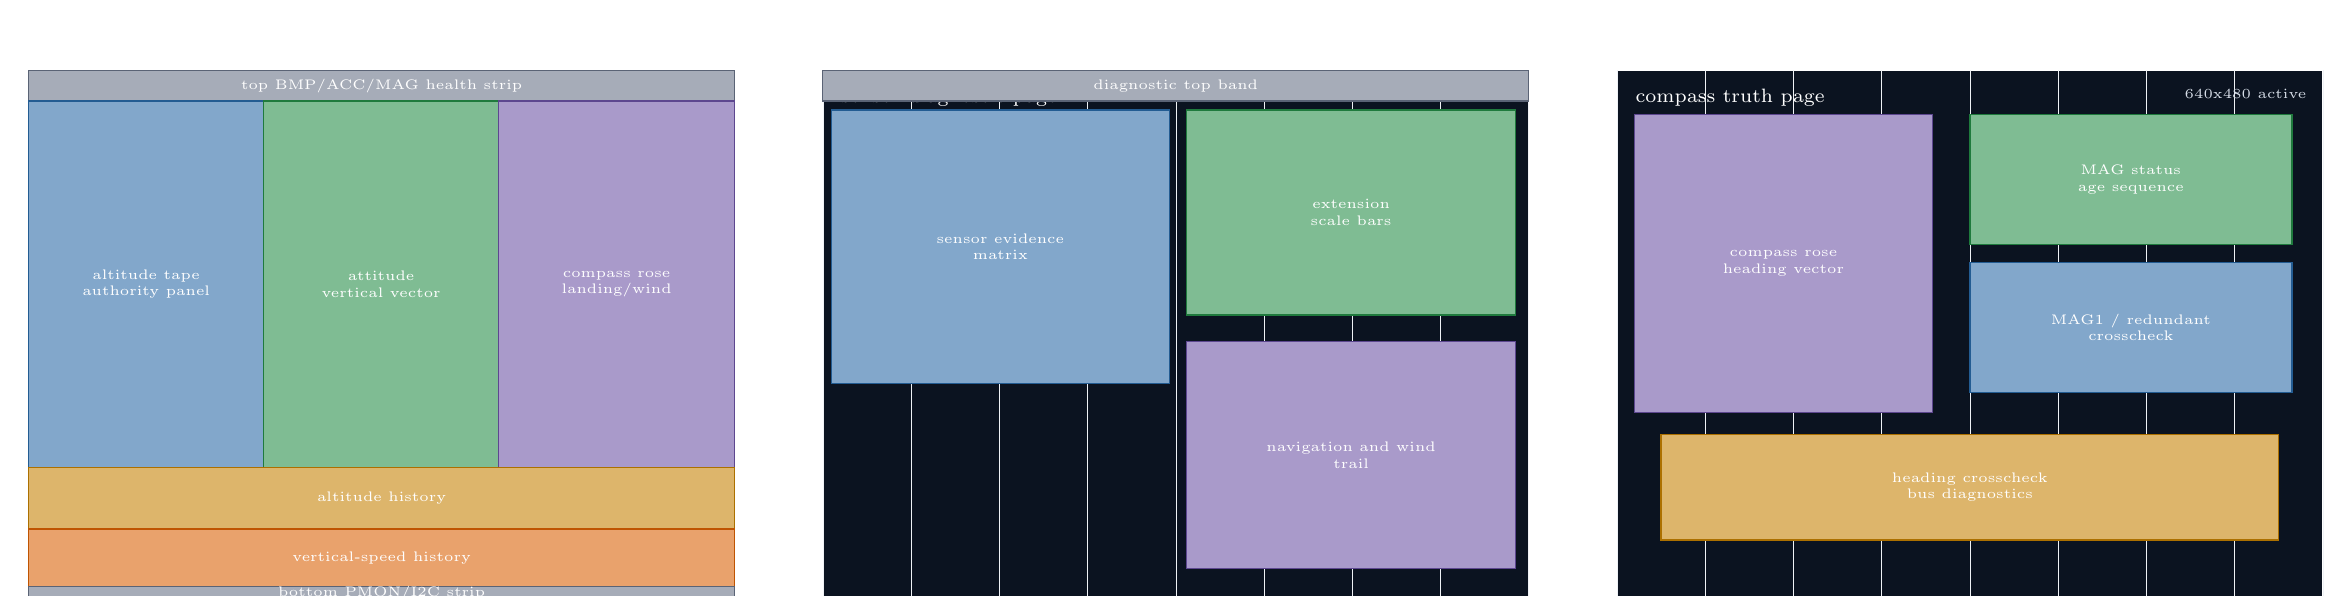
\begin{tikzpicture}[x=0.014cm,y=-0.014cm]
  \begin{scope}
    \screenframe{normal flight HUD / self-test HUD}
    \screenrect{0}{0}{640}{28}{CFGray}{top BMP/ACC/MAG health strip}
    \screenrect{0}{28}{213}{332}{CFBlue}{altitude tape\\authority panel}
    \screenrect{213}{28}{213}{332}{CFGreen}{attitude\\vertical vector}
    \screenrect{426}{28}{214}{332}{CFPurple}{compass rose\\landing/wind}
    \screenrect{0}{360}{640}{56}{CFAmber}{altitude history}
    \screenrect{0}{416}{640}{52}{CFOrange}{vertical-speed history}
    \screenrect{0}{468}{640}{12}{CFGray}{bottom PMON/I2C strip}
  \end{scope}

  \begin{scope}[shift={(720,0)}]
    \screenframe{sensor diagnostic page}
    \screenrect{8}{36}{306}{248}{CFBlue}{sensor evidence\\matrix}
    \screenrect{330}{36}{298}{186}{CFGreen}{extension\\scale bars}
    \screenrect{330}{246}{298}{206}{CFPurple}{navigation and wind\\trail}
    \screenrect{0}{0}{640}{28}{CFGray}{diagnostic top band}
  \end{scope}

  \begin{scope}[shift={(1440,0)}]
    \screenframe{compass truth page}
    \screenrect{16}{40}{270}{270}{CFPurple}{compass rose\\heading vector}
    \screenrect{320}{40}{292}{118}{CFGreen}{MAG status\\age sequence}
    \screenrect{320}{174}{292}{118}{CFBlue}{MAG1 / redundant\\crosscheck}
    \screenrect{40}{330}{560}{96}{CFAmber}{heading crosscheck\\bus diagnostics}
  \end{scope}
\end{tikzpicture}}
\caption[Screen layout arrangements]{Screen layout arrangements for the primary HUD/self-test HUD, sensor diagnostic page, and optional compass truth page.  Coordinates are active VGA pixels with origin at the upper-left.}
\label{fig:layouts}
\end{figure}
\clearpage

\section{Color Conventions}

The renderer uses 12-bit RGB444 colors.  Color is not decoration; it encodes
data health, provenance, and warning state.

\begin{table}[H]
\caption{Semantic color conventions.}
\label{tab:colors}
\small
\begin{tabularx}{\linewidth}{L{0.20\linewidth} L{0.22\linewidth} Y}
\toprule
\textbf{Color family} & \textbf{Typical RGB444 examples} & \textbf{Meaning} \\
\midrule
Black and dark grid & \sig{12'h000}, \sig{12'h011}, \sig{12'h111} & Inactive video, background, grid, panel separation. \\
White and gray & \sig{12'hFFF}, \sig{12'hAAA}, \sig{12'h666} & Text, neutral geometry, stale/unavailable secondary markings. \\
Green & \sig{12'h2B5}, \sig{12'h143}, \sig{12'h154} & Valid, fresh, healthy, reachable, or nominal state. \\
Yellow/amber & \sig{12'hD93}, \sig{12'hFD0}, \sig{12'hFC2} & Valid but stale, warning, marginal, or inspection state. \\
Orange/red & \sig{12'hF50}, \sig{12'hF80}, \sig{12'hD33} & Invalid, faulted, rejected, alert, or out-of-policy condition. \\
Cyan/blue/purple & \sig{12'h3FF}, \sig{12'h86F}, \sig{12'h426} & Heading, vector, authority envelope, or diagnostic emphasis. \\
\bottomrule
\end{tabularx}
\end{table}

\section{Compositor Layer Behavior}

The implemented layer stack is intentionally deterministic.  A higher layer
dominates a lower layer only under its explicit enable condition.  The sensor
diagnostic page is selected before the normal HUD text overlay, so primary HUD
labels do not occlude diagnostic matrices.

\begin{figure}[H]
\centering
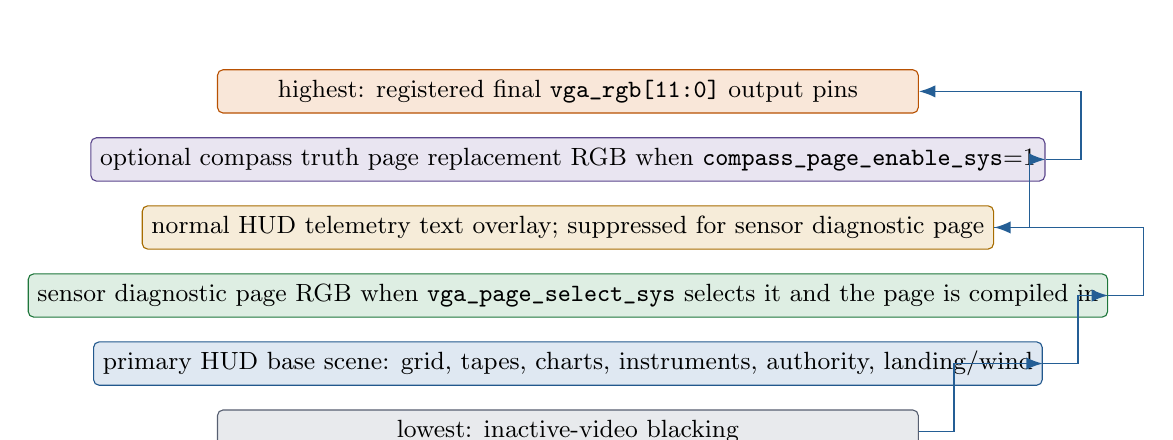
\begin{tikzpicture}[node distance=0.30cm]
  \node[cfLayer=CFGray] (black) {lowest: inactive-video blacking};
  \node[cfLayer=CFBlue, above=of black] (base) {primary HUD base scene: grid, tapes, charts, instruments, authority, landing/wind};
  \node[cfLayer=CFGreen, above=of base] (diag) {sensor diagnostic page RGB when \sig{vga_page_select_sys} selects it and the page is compiled in};
  \node[cfLayer=CFAmber, above=of diag] (text) {normal HUD telemetry text overlay; suppressed for sensor diagnostic page};
  \node[cfLayer=CFPurple, above=of text] (truth) {optional compass truth page replacement RGB when \sig{compass_page_enable_sys}=1};
  \node[cfLayer=CFOrange, above=of truth] (pins) {highest: registered final \sig{vga_rgb[11:0]} output pins};

  \draw[cfArrow] (black.east) -- ++(0.45,0) |- (base.east);
  \draw[cfArrow] (base.east) -- ++(0.45,0) |- (diag.east);
  \draw[cfArrow] (diag.east) -- ++(0.45,0) |- (text.east);
  \draw[cfArrow] (text.east) -- ++(0.45,0) |- (truth.east);
  \draw[cfArrow] (truth.east) -- ++(0.45,0) |- (pins.east);
\end{tikzpicture}
\caption[Compositor layer stack]{Compositor layer stack.  The stack is deterministic: inactive video is black, selected page RGB forms the base visible page, normal text overlays only the primary HUD, and the optional compass truth page replaces the HUD stream when selected.}
\label{fig:layers}
\end{figure}

\section{Telemetry Fields by Mode}

\begin{longtable}{L{0.19\linewidth} L{0.73\linewidth}}
\caption{Telemetry fields shown in each mode.}
\label{tab:telemetry-by-mode}\\
\toprule
\textbf{Mode} & \textbf{Fields and visible evidence} \\
\midrule
\endfirsthead
\toprule
\textbf{Mode} & \textbf{Fields and visible evidence} \\
\midrule
\endhead
Normal flight HUD &
Top strip: BMP, ACC, MAG validity, status, age, and sequence.  Left column:
roll, roll freshness, accelerometer reference validity, accelerometer age and
sequence, and derived-ACC provenance.  Middle column: altitude, vertical speed,
altitude/vertical-speed freshness, derived validity, BMP reference validity,
BMP age and sequence.  Right column: heading, heading freshness, MAG reference
validity, MAG age and sequence, and derived-MAG provenance.  Bottom strip:
PMON voltage/current code, alert flags, age, sequence, I2C NACK count, and I2C
timeout count.  Base scene also shows authority phase/gates, target envelopes,
navigation/wind viewport, and altitude/vertical-speed history. \\
Self-test HUD &
Same visible fields as normal flight HUD, but the upstream visualization suite
selects self-test stimulus through \sig{flight_selftest_en_sys}.  This mode is
therefore a renderer and compositor checkout rather than live-sensor evidence. \\
Sensor diagnostic page &
Sensor matrix rows for BMP, ACC, MAG, PWR, derived, extension, navigation, and
wind evidence.  Each row emphasizes validity, status, age/freshness, and fault
state.  Extension scale bars cover MAG delta/norm evidence, range height, air
differential pressure and speed, environment temperature/humidity, sun luma,
flow magnitude, log sequence/drop, and maximum age.  Lower-right viewport shows
current and recent navigation/wind points. \\
Compass truth page &
MAG heading page fields: planar heading vector, compass rose, MAG validity,
status, age, sequence, raw magnetic-field evidence, MAG1/redundant evidence,
heading crosscheck, and protocol/bus diagnostics. \\
\bottomrule
\end{longtable}

\section{Default and Fallback Behavior}

\begin{longtable}{L{0.26\linewidth} L{0.31\linewidth} L{0.33\linewidth}}
\caption{Default and fallback display behavior.}
\label{tab:fallbacks}\\
\toprule
\textbf{Condition} & \textbf{Implemented response} & \textbf{Reason} \\
\midrule
\endfirsthead
\toprule
\textbf{Condition} & \textbf{Implemented response} & \textbf{Reason} \\
\midrule
\endhead
Reset with source-default parameters &
Registered view resets to \sig{VIEW_FLIGHT_HUD}. &
Boots into the always-present primary HUD. \\
Compass-default parameter set and compass page compiled in &
Registered reset view can be compass truth page. &
Supports a MAG/heading diagnostic build without changing operator controls. \\
Illegal reset view ID &
Reset view is coerced to \sig{VIEW_FLIGHT_HUD}. &
Prevents booting into an undefined display state. \\
Illegal direct view ID &
Current selected view is held and \sig{cfg_invalid_view_sys} is latched. &
Configuration errors are observable in RTL without corrupting visible output. \\
Compass page request while page is compiled out &
Direct request is rejected; legacy compass hold has no effect on the absent page. &
Avoids a blank or unreachable renderer path. \\
Sensor diagnostic view while page is compiled out &
The registered view remains legal, but the visible renderer falls back to primary
HUD RGB. &
Allows navigation-state verification without carrying optional page LUT cost. \\
Inactive video interval &
\sig{vga_rgb} is forced black. &
Keeps blanking deterministic and monitor-friendly. \\
Telemetry invalid, stale, or unavailable &
Fields remain visible with red, yellow/amber, gray, or placeholder semantics. &
The display remains an engineering instrument instead of hiding failures. \\
\bottomrule
\end{longtable}

\section{Debug Views and Operational Use}

\begin{table}[H]
\caption{Recommended use of each display view during bring-up and debugging.}
\label{tab:debug-use}
\small
\begin{tabularx}{\linewidth}{L{0.24\linewidth} Y}
\toprule
\textbf{View} & \textbf{Use during development} \\
\midrule
\sig{VIEW_FLIGHT_HUD} & Use first to verify sync, RGB output, default rendering, live telemetry publication, SYS-to-PIX CDC, and frame-stable visual updates. \\
\sig{VIEW_SELFTEST_HUD} & Use when live telemetry is absent or suspect; validates renderer geometry, layer order, text placement, history drawing, and color paths. \\
\sig{VIEW_SENSOR_DIAG} & Use for sensor integration and stale/fault triage.  It is the highest-density view for validity, age, status, extension presence, and navigation/wind evidence. \\
\sig{VIEW_COMPASS_TRUTH} & Use for MAG/heading checkout.  It isolates planar heading evidence, MAG status, redundant MAG1 comparison, and bus diagnostics from the normal HUD. \\
\bottomrule
\end{tabularx}
\end{table}

\section{Known Rendering Limitations}

\begin{longtable}{L{0.26\linewidth} L{0.36\linewidth} L{0.28\linewidth}}
\caption{Known rendering limitations and engineering impact.}
\label{tab:limitations}\\
\toprule
\textbf{Limitation} & \textbf{Current condition} & \textbf{Impact} \\
\midrule
\endfirsthead
\toprule
\textbf{Limitation} & \textbf{Current condition} & \textbf{Impact} \\
\midrule
\endhead
Resource-constrained optional pages &
The compass truth page is off by default in the Basys-3 configuration, while
the lighter in-HUD sensor diagnostic page is enabled by default. &
Compass-page-enabled builds require separate synthesis/implementation evidence. \\
No anti-aliased text &
The text compositor uses compact fixed glyphs. &
Labels are deterministic and cheap, but long labels must be abbreviated. \\
Fixed layout &
Viewport coordinates are compile-time constants. &
No runtime zoom, pan, rearrangement, or automatic layout adaptation. \\
RGB444 output &
Only 4 bits per color channel are driven. &
Fine gradients and subtle diagnostic shading are intentionally limited. \\
No explicit board data-enable pin &
Active video exists inside the renderer; the board exposes sync and RGB only. &
Any future digital-video bridge must derive data-enable from the same timing
contract. \\
Limited view-state observability &
\sig{view_effective_sys} and \sig{cfg_invalid_view_sys} are not yet routed to a
visible board/debug channel. &
Bench validation of rejected view IDs and hold priority currently requires RTL
simulation or added debug wiring. \\
Encoded selector switch reuse &
The encoded-view selector reuses SW11--SW13, which also drive MAG1
bench offsets and diagnostic fault-class bits. &
RTL arbitration gives ownership to MAG1 bench mode and SW2+SW6 diagnostic fault
injection.  BTNR requests during those ownership modes force reserved ID
\bits{3'b111}, preserve \sig{view_sel_sys}, and latch
\sig{cfg_invalid_view_sys}; a future switch bank would still be cleaner for
operator-facing builds. \\
\bottomrule
\end{longtable}

\section{Verification Checklist}

\begin{longtable}{L{0.30\linewidth} L{0.58\linewidth}}
\caption{Recommended verification checklist for this rendering control map.}
\label{tab:verification}\\
\toprule
\textbf{Check} & \textbf{Expected evidence} \\
\midrule
\endfirsthead
\toprule
\textbf{Check} & \textbf{Expected evidence} \\
\midrule
\endhead
View traversal &
Simulation proves next/previous order, compass-page skip when compiled out,
and direct compass selection when compiled in. \\
Switch-encoded direct traversal &
Focused render-control simulation shows SW13:SW11 encodings \bits{000} through
\bits{110} select or reject the expected view when BTNR is pressed with SW3 low
and SW2+SW6 fault injection inactive; reserved \bits{111}, SW3 MAG1-bench
ownership, and SW2+SW6 fault-injection ownership leave \sig{view_sel_sys}
unchanged and latch \sig{cfg_invalid_view_sys}. \\
Illegal direct selection &
Illegal view IDs leave \sig{view_sel_sys} unchanged and latch
\sig{cfg_invalid_view_sys}. \\
Legacy hold priority &
SW4/SW14 compass hold overrides registered view when the page exists; SW2
self-test hold overrides registered view below compass hold priority. \\
Sensor diagnostic fallback &
\sig{VIEW_SENSOR_DIAG} produces diagnostic RGB when compiled in and primary HUD
RGB when compiled out. \\
Layer priority &
Text overlays primary HUD only, does not occlude the sensor diagnostic page,
and optional compass truth replacement dominates the HUD stream when enabled. \\
Frame stability &
View changes and semantic bundle updates do not tear within a visible frame. \\
Implementation evidence &
Record utilization, timing, DRC, and bitstream hash for source-default and
optional page-enabled builds. \\
Bench evidence &
Capture reset/default HUD, self-test HUD, sensor diagnostic page if compiled,
compass truth page if compiled, stale/error color behavior, and inactive-video
black level. \\
\bottomrule
\end{longtable}

\section{Recommended Next Development Steps}

\begin{enumerate}
  \item Keep \file{tb_caelumfusion_render_control_switch_encoded.v} in the
        regression flow and add a one-command Tcl runner for the focused
        switch-encoded view-selection test.
  \item Route \sig{view_effective_sys}, \sig{view_sel_sys}, and
        \sig{cfg_invalid_view_sys} to a small visible debug field, LEDs, or UART
        status for bench validation.
  \item Build and archive three bitstreams: source-default HUD, compass-truth
        enabled, and sensor-diagnostic enabled.  Record utilization, WNS/WHS,
        DRC status, and bitstream hashes.
  \item Capture VGA evidence for each view and annotate the capture with switch
        positions, compile-time parameters, and the programmed bitstream hash.
\end{enumerate}

\section{Conclusion}

The CaelumFusion display system is a VGA-only Basys-3 rendering path with a
small deterministic view selector and a fixed, source-grounded compositor.  The
default display is the primary flight HUD; self-test uses the same renderer with
synthetic stimulus; the sensor diagnostic page is a page-selectable HUD-renderer
mode; and the compass truth page is an optional full-screen replacement overlay.
The design preserves deterministic behavior under disabled options, invalid
view requests, stale telemetry, and inactive-video intervals.  The remaining
engineering work is not conceptual definition but verification: exercise the
view selector, expose view state for bench debug, and record implementation and
VGA capture evidence for each build variant.

\end{document}
